\documentclass[aps,prd,amsmath,amssymb,showpacs,floats,floatfix,nofootinbib,reprint]{revtex4-1}
%\documentclass[10pt,aps,prd,amsmath,amssymb,showpacs,floats,floatfix,nofootinbib,twocolumn]{revtex4}
%%compile with pdflatex or xelatex%%
%aps: The style refers to a journal of the APS (Amercian Physical Society) family
%prl/prd: The journal shall be Physical Review Letters/Physical Review D (shortened PRL/PRD)
%reprint: Print the document with two columns as it would be printed in the journal.
%preprint: Another option which would print the document with single column as larger line spread for proofreading purposes.
\usepackage[colorlinks=true, linkcolor=red, citecolor=blue,CJKbookmarks=true]{hyperref}
\usepackage{amsmath,amsfonts,amssymb}
\usepackage{graphicx}
\usepackage{color}
\usepackage[dvipsnames,svgnames,x11names]{xcolor}
\usepackage{slashed} % slash mark
\usepackage{url}
\usepackage{subfigure}
\usepackage{multirow} % multirows in tabular environment
\usepackage{setspace} % spacing
\graphicspath{{figs/}}  % figure path
\setcounter{MaxMatrixCols}{30}
\def\red#1{{\textcolor{red}{#1}}} % red color

\makeatother
\allowdisplaybreaks % allow eqnarray breaks
\begin{document}

\setstretch{1.2} % line spacing

\title{results and discussion} 

%\maketitle


\begin{figure*}%[!htbp]
\caption{\textbf{\red{Decay}}. Comparison of the limits on decay lifetime set by LHAASO and HAWC for different $D$-factors.}
%{\includegraphics[width=0.3\textwidth]{comparison_bootes.eps}}
%{\includegraphics[width=0.3\textwidth]{comparison_hercules.eps}}
%{\includegraphics[width=0.3\textwidth]{comparison_leo1.eps}}
{\includegraphics[width=0.3\textwidth]{comparison_segue1.eps}}
{\includegraphics[width=0.3\textwidth]{comparison_comab.eps}}
{\includegraphics[width=0.3\textwidth]{comparison_trian2.eps}}
{\includegraphics[width=0.3\textwidth]{comparison_draco.eps}}
{\includegraphics[width=0.3\textwidth]{comparison_urmajor2.eps}}
{\includegraphics[width=0.3\textwidth]{comparison_urminor.eps}}
\label{fig:dsph-comparison}
\end{figure*}

\begin{figure*}[!htbp]
\caption{\textbf{\red{Decay}}. Comparison for the same $D$-factors.}
%{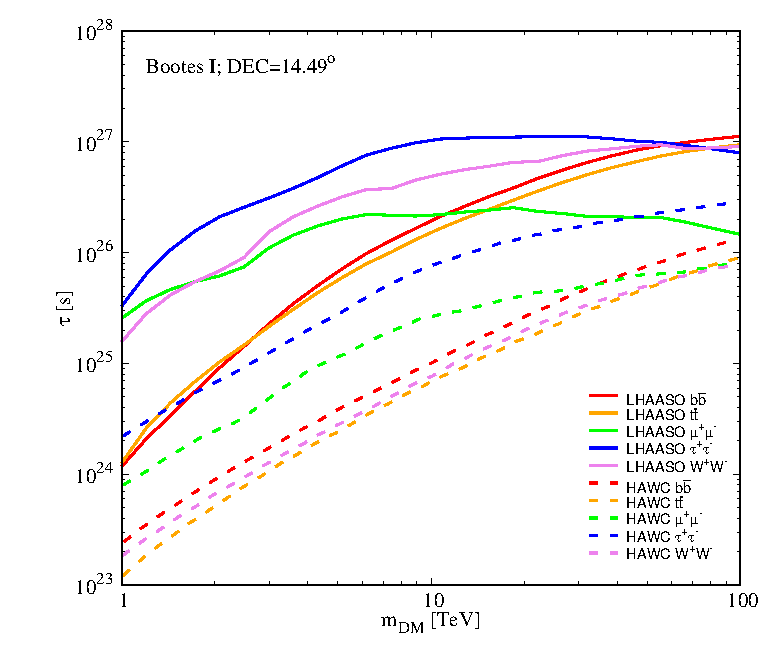
\includegraphics[width=0.3\textwidth]{comparison_bootes-hawc.eps}}
%{\includegraphics[width=0.3\textwidth]{comparison_hercules-hawc.eps}}
%{\includegraphics[width=0.3\textwidth]{comparison_leo1-hawc.eps}}
%{\includegraphics[width=0.3\textwidth]{comparison_leo2-hawc.eps}}
{\includegraphics[width=0.3\textwidth]{comparison_segue1-hawc.eps}}
{\includegraphics[width=0.3\textwidth]{comparison_comab-hawc.eps}}
{\includegraphics[width=0.3\textwidth]{comparison_trian2-hawc.eps}}
{\includegraphics[width=0.3\textwidth]{comparison_draco-hawc.eps}}
{\includegraphics[width=0.3\textwidth]{comparison_urmajor2-hawc.eps}}
{\includegraphics[width=0.3\textwidth]{comparison_urminor-hawc.eps}}
\end{figure*}


\begin{figure*}%[!htbp]
\caption{\red{\bf Annihilation}. Comparison of the limits set by LHAASO and HAWC for different $J$-factors.}
{\includegraphics[width=0.3\textwidth]{comparison_segue1-ani.eps}}
{\includegraphics[width=0.3\textwidth]{comparison_comab-ani.eps}}
{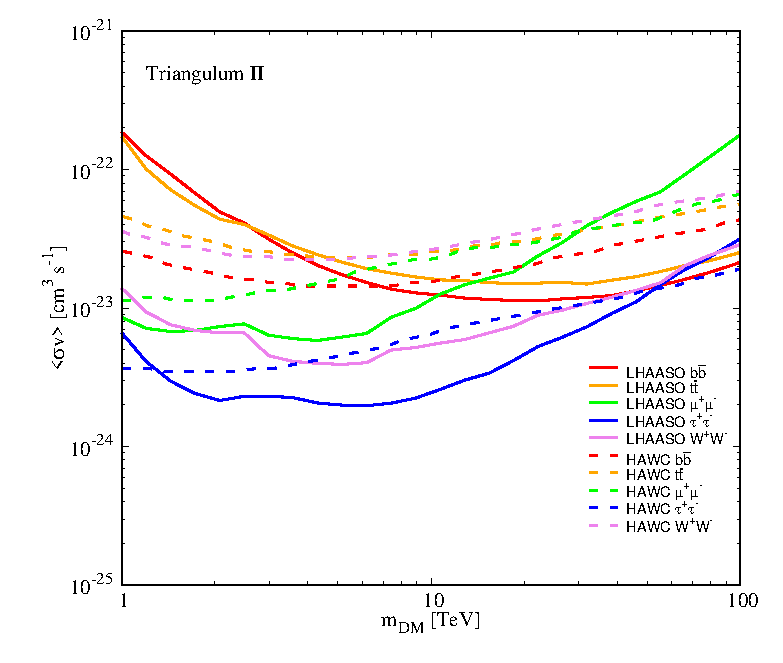
\includegraphics[width=0.3\textwidth]{comparison_trian2-ani.eps}}
{\includegraphics[width=0.3\textwidth]{comparison_draco-ani.eps}}
{\includegraphics[width=0.3\textwidth]{comparison_urmajor2-ani.eps}}
{\includegraphics[width=0.3\textwidth]{comparison_urminor-ani.eps}}
\end{figure*}

\begin{figure*}%[!htbp]
\caption{\red{\bf Annihilation}. Comparison for the same $J$-factors.}
{\includegraphics[width=0.3\textwidth]{comparison_segue1-hawc-ani.eps}}
{\includegraphics[width=0.3\textwidth]{comparison_comab-hawc-ani.eps}}
{\includegraphics[width=0.3\textwidth]{comparison_trian2-hawc-ani.eps}}
{\includegraphics[width=0.3\textwidth]{comparison_draco-hawc-ani.eps}}
{\includegraphics[width=0.3\textwidth]{comparison_urmajor2-hawc-ani.eps}}
{\includegraphics[width=0.3\textwidth]{comparison_urminor-hawc-ani.eps}}
\end{figure*}

\input{dsph}
\begin{figure*}
\includegraphics[scale=0.8]{dnde}
\end{figure*}

\begin{figure*}%[!htbp]
\caption{Combined annihilation.}
{\includegraphics[width=0.45\textwidth]{annihilate_combined_bottom.eps}}
{\includegraphics[width=0.45\textwidth]{annihilate_combined_top.eps}}
{\includegraphics[width=0.45\textwidth]{annihilate_combined_mu.eps}}
{\includegraphics[width=0.45\textwidth]{annihilate_combined_tau.eps}}
{\includegraphics[width=0.45\textwidth]{annihilate_combined_ww.eps}}
\end{figure*}

\begin{figure*}%[!htbp]
\caption{Combined decay.}
{\includegraphics[width=0.45\textwidth]{decay_combined_bottom.eps}}
{\includegraphics[width=0.45\textwidth]{decay_combined_top.eps}}
{\includegraphics[width=0.45\textwidth]{decay_combined_mu.eps}}
{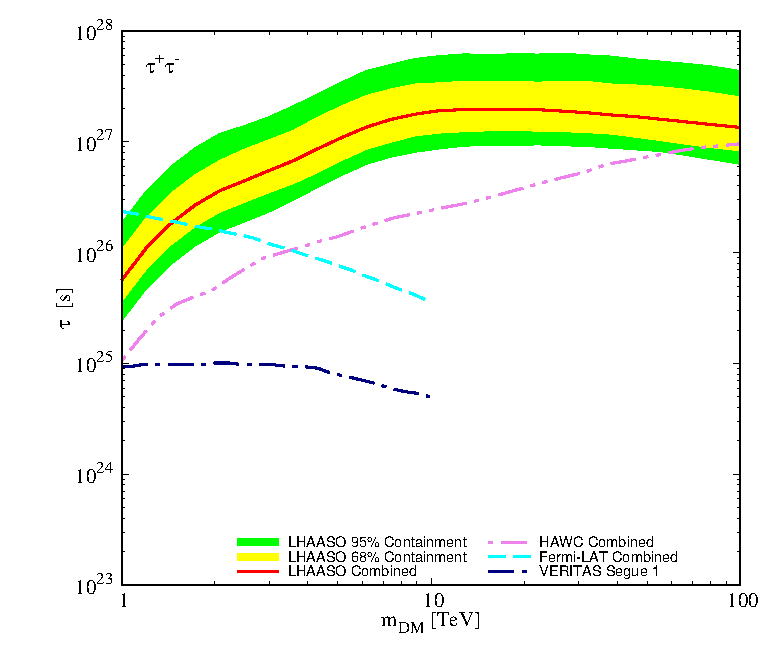
\includegraphics[width=0.45\textwidth]{decay_combined_tau.eps}}
{\includegraphics[width=0.45\textwidth]{decay_combined_ww.eps}}
\end{figure*}
\end{document}